Wang et al. \cite{wangSSAformerSpatialSpectral2024} propose the Spatial-Spectral Aggregation Transformer (SSAformer),
for the task of hyperspectral image super resolution.
Similarly to the Hybrid Attention Transformer introduced by Chen et al. \cite{chenHATHybridAttention2024},
the Spectral-Spatial Attention Block, 
the basic building block of the SSAformer architecture,
employs channel attention and overlapping cross-attention in parallel.
This design is motivated by the need to comprehensively fuse spatial and spectral information, 
overcoming the limitations of CNNs’ locality and conventional Transformers’ imbalance between the two domains.
The architecture is visualized in figure \ref{fig:ssaformer}.

\begin{figure}[h!]
    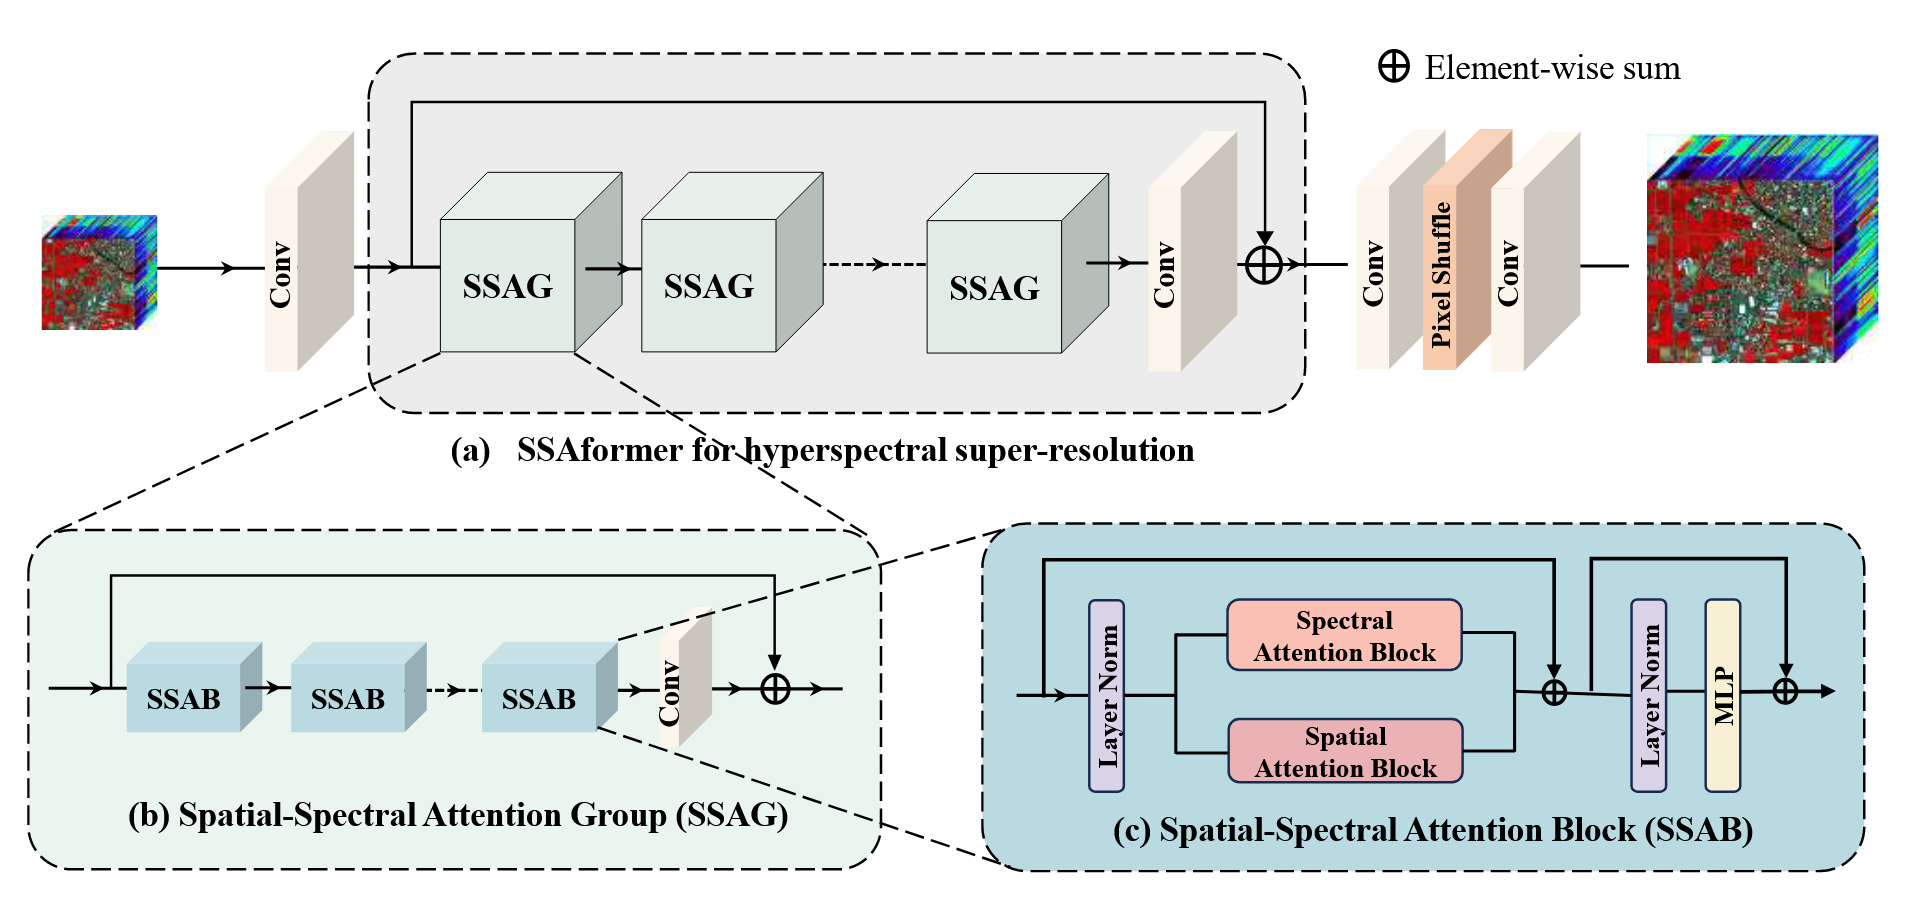
\includegraphics[width=0.9\textwidth]{models/hsisr/imgs/ssaformer.png}
    \caption{Image taken from \cite{zhangImageSuperResolutionUsing2018}, architecture of RCAB module.}
    \label{fig:ssaformer}
\end{figure}

For initial feature extraction a single convolutional layer is used.
To scale features to the desired size, a sub-pixel convolution is performed.

\noindent The deep feature extraction module $H_d$ is composed of $4$ Spatial-Spectral Attention Groups (SSAGs),
followed by a final convolutional layer

    $$ H_d = C \circ H_{SSAG} \circ ... \circ H_{SSAG} ~. $$

A SSAG is formed by $4$ Spectral-Spatial Attention Blocks (SSABs), succeeded as well by convolutional layer

    $$ H_{SSAG} = C \circ H_{SSAB} \circ ... \circ H_{SSAB} ~.$$

The SSAB forms the basic building block of the architecture proposed by Wang et al. \cite{wangSSAformerSpatialSpectral2024}.
Overlapping Cross-Attention is employed in parallel,
to a Channel Attention Block $H_{CAB}$, defined in equation (\ref{eq:cab})

    $$ H_{SSAB} = R(\Phi \circ \text{LN}) \circ R(s \circ P( \text{OCA}(180, 6), H_{CAB}) \circ \text{LN}) ~, $$

where $\Phi:180 \to 180$ is a neural network, the architecture is not specified by the authors.
Again, a model as in equation (\ref{eq:phi}) could be used.